\begin{figure}[htb]
    \centering
    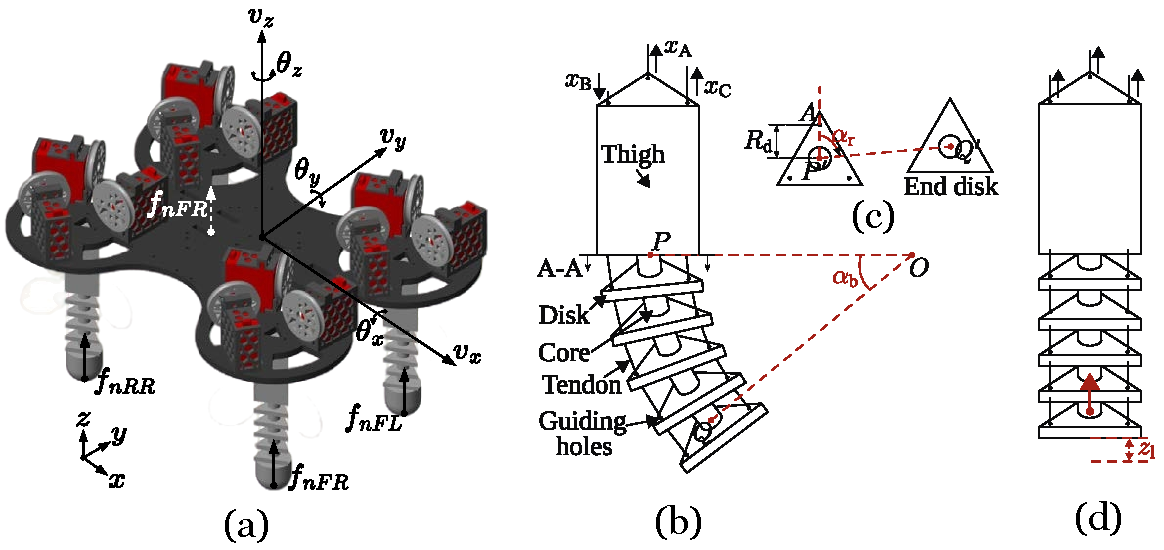
\includegraphics[width=\linewidth]{img/chap3/robots.pdf}
    \caption{Graphical overview of SoftQ and the Compressible Tendon-driven Soft Actuator (CTSA) to drive the robot. (a) Rendered robot with key state notations. (b) The structure and notations of the CTSA. The upper part from section A-A is the rigid thigh for maintaining the actuator length and the lower part is compressible and bendable. The bending angle of the lower part is noted as $\alpha_b$. (c) The top view of the bent CTSA of section A-A. $\alpha_r$ refers to the rotational angle of the CTSA. (d) The CTSA compression is realized by pulling the three tendons by the same amount, with the compression length being noted as $z_l$, originated from Ji et al.\cite{jiSynthesizingOptimalGait2022, jiOmnidirectionalWalkingQuadruped2022}}
    \label{fig:robot}
\end{figure}